\section{Organisational Breakdown Structure (OBS)}\label{cha:OBS}
In this chapter the organisational breakdown structure is illustrated and explained. The breakdown can be considered as two separate parts. The first is the management breakdown, which shows the responsibilities of the various roles and is discussed in the first section. The second section deals with the engineering breakdown. Given in Figure \ref{fig:OBS} is the OBS, where every position will be explained in more detail in sections \ref{subsec:management} and \ref{subsec:engineer}.

\begin{figure}[h]
\centering
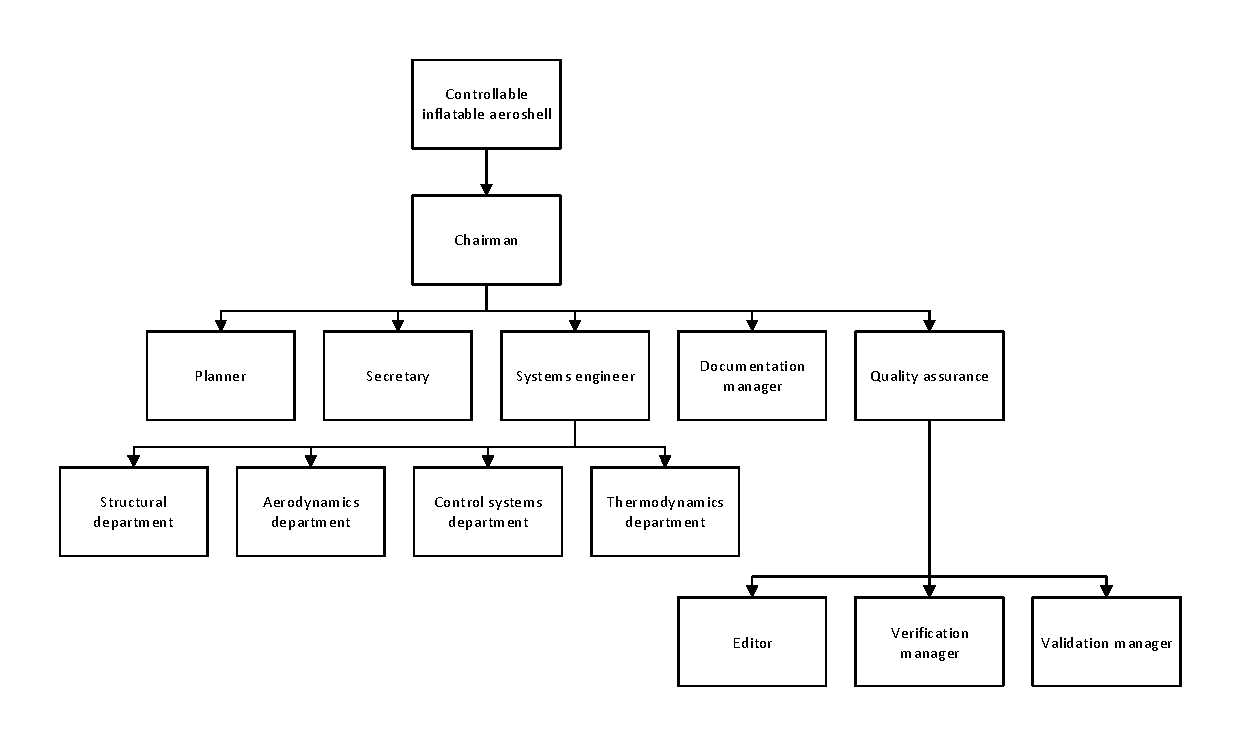
\includegraphics[width=0.95\textwidth]{./Figure/OBS.pdf}
\caption{Organisational breakdown structure} \label{fig:OBS}
\end{figure}

\subsection{Management breakdown}\label{subsec:management}
% Organisational Breakdown Structure (organogram with the responsibilities of the various group members)
The size of the project group, with nine people, is too large to be self-organizing: if no organizational structure is apparent, people will not have a clear view of the required work, leading to inefficient time-management. Therefore the organization is broken down into different positions with corresponding responsibilities. All positions do not entail exclusive contribution of the appointed functions, but indicate where final responsibility lies for each aspect. Therefore team members assist and communicate with one another between different management functions.


\subsubsection{Chairman}\label{subsec:Chairman}
The size of the DSE project group, with 9 people, is too large to be self-organizing: if no organizational structure is apparent, people will not have a clear view of the required work, leading to inefficient time-management. The role of the chairman is to prepare team meetings and guide them such that the meeting itself is performed in an efficient manner, but also the goal of the meeting is achieved: at the end of the meeting, all team members should have a clear overview of the current status of the project, as well as their present responsibilities. It is the task of the chairman to guide meetings such that this information is conveyed between the team members including the members responsible for planning, documentation, and the system engineer. Concretely, this also encompasses making the agenda.

\subsubsection{Secretary}\label{subsec:Secretary}
	The secretary shall minute during both project and customer meetings and keep track of design decisions and how they are made. This is done to assure that changes in the design process can be reviewed and remember why changes are made the way they are made. Furthermore, the secretary shall be responsible for all internal and external communication.

\subsubsection{Documentation manager}\label{subsec:D_and_A}
One of the tasks of the documentation manager is to maintain a structure in the file system used on the computer (i.e. keeping Dropbox and Github organized). The documentation manager is also the person to set up the initial files (like the LaTeX templates) and folder structures. The documentation manager should provide basic rules for the layout of the documents, communication with the editor is needed when the layout does not conform these rules. It is needed that this structure is maintained throughout the project and group members should make an effort to keep it this way, if not it is the documentation manager that will point out these problems towards the group and come with possible solutions. 

\subsubsection{Planner}\label{subsec:Planner}
The planner provides an overview for all the work packages as progressing through to time in the form of a Gantt chart. It is the function of the planner to frequently update and further detail this chart throughout the progress of the project. Furthermore more the planner is required to communicate all deadlines to the group members. Interactions between different tasks are provided and planning is made accordingly to allow all tasks to be finished before the set deadlines or milestones. Progression is recorded throughout the process to ascertain that all deadlines are met. 



\subsubsection{Systems engineer}\label{subsec:SE}
The systems engineer is responsible for the overall technical progress of the project. He keeps track of the project requirements and manages the interfaces between different design disciplines. His responsibilities can be summarized as follows:

\begin{itemize}
\item Track project requirements and overall technical progress
\item Manage design interfaces between design disciplines
\item Resolve design conflicts due to conflicting requirements 
\end{itemize}


\subsubsection{Risk Engineer}\label{subsec:RiskEng}
To mitigate cost or time overruns or even worse, eventual product failure, risk management plays a central role within project management. In order to properly address the risks involved in developing an inflatable aeroshell one person is ultimately responsible for possible hazard management: The risk engineer. The task of this risk engineer is to manage the various risks encountered during the design process. This will be done by using technical budgeting to manage the performance risks during the various design phases. Performance margins can be defined for each system and subsystem that influence the performances of other systems. In addition to this risk mapping will be used. By identifying critical components of each proposed concept and allocating the available resources accordingly the project risks can be minimized. Risk management is a continuous process.

\subsubsection{Quality assurance}\label{subsec:QA}
\paragraph{Editor}
Primary function is assuring consistent and high quality of all written communication, by means of proof-reading and correcting of pieces submitted by all group members. In addition, the lay-out and structure of reports and presentations is scrutinized and egalized. Strong interaction takes place with all group members with direct contributions to the written work, while open communication with documentation manager is maintained to resolve issues with the formatting of reports. In case of repeated errors by group members, the editor makes an effort to enter conversation with the repeaters in order to identify the origin of the problem and if need be to take pre-emptive action against future occurrences.
\paragraph{Verification}
Verification occurs at multiple stages of the design. For one, concepts should be verified to check whether the developed product meets the requirements. The team member in charge of verification

\paragraph{Validation}
IEEE defines validation as ''The assurance that a product, service, or system meets the needs of the customer and other identified stakeholders. It often involves acceptance and suitability with external customers.''(ref. ''IEEE V\&V.pdf'') The person in charge of validation is thus responsible for the compliance of the product with the requirements imposed by the costumers and stakeholders. Another task is to assure that the subsystem requirements contribute to accomplishing the system requirements and in the end to the top level requirements.


\subsection{Engineering breakdown}\label{subsec:engineer}
The engineering work of the controllable inflatable aeroshell is divided into different departments. These departments are the driving fields in the design of an inflatable aeroshell and will cover all aspects of the design. As for the management positions, engineering departments are not isolated in the sense that the aim is to involve team members in multiple design aspects.

\subsubsection{Aerodynamics department}\label{subsec:aero}
The aerodynamics department will look at different shapes possible to do the entry in the Martian atmosphere. This department looks at the hypersonic aerodynamics and determine the amount of thermal energy the heat shield needs to absorb and the loads that the structure needs to endure. One of the other aspects will the creation of a aerodynamic model of the vehicle that will be used in the control system.

\subsubsection{Structures department}\label{subsec:struct}
The structures department is responsible for the design of the structure, carrying primarily the mechanical and thermal loads by aerodynamic forces and heating. This design entails appropriate material selection, design and sizing of load-carrying elements and integrating the design while maintaining feasibility in terms of manufacturability, costs and weight. For the purpose of determining structural performance, the structures department is responsible for the development of structural tools. Moreover, the structures department actively communicates with other departments to synthesize the system design.

\subsubsection{Control systems department}\label{subsec:control}
The control systems department will analyse the controllability and stability (C \& S), both static and dynamic, of the vehicle. Further this department will design the subsystems that will provide the needed characteristics for the C \& S. The department covers all additional subsystems to ensure the C \& S system to be fully functional, i.e. an attitude determination system.


\subsubsection{Thermal control department}\label{subsec:therm}
The thermodynamics department will look at the thermal aspect of the inflatable aeroshell. The aerodynamics department will provide a boundary condition for the heat propegation within the structure. This heat propegation will be dependent on the material properties and structure shape as defined by the structures department. Furthermore, the spacevehicle should have a thermal control such that systems can operate and humans can survive.